% !TEX TS-program = pdflatex
% !TEX root = ../ArsClassica.tex

%************************************************
\chapter{Heuristic Methods}
\label{chp:5-Heuristic}
%************************************************
As we already said, our problem belongs to the class of NP-Hard problems. Therefore, when the number of nodes is too high, we cannot expect to always obtain an optimal solution in a short amount of time.
For this reason we have decided to implement some algorithms that, instead of solving the mathematical model, use heuristic methods to find a solution of the problem. These methods, relying on the characteristic structure of the problem,  can compute  quickly a good solution that is not guaranteed to be optimal.
Then, in the following section, we will describe some heuristic methods that iteratively execute a specific procedure trying to obtain better and better solutions.
\section{Prim-Dijkstra}
The Prim-Dijkstra algorithm was developed in 1930 by Czech mathematician Vojtěch Jarník and later rediscovered and republished by computer scientists Robert C. Prim in 1957 and Edsger W. Dijkstra in 1959.\\
In computer science, Prim's algorithm is a greedy algorithm that finds a minimum spanning tree for a weighted undirected graph. This means that it finds a subset of the edges that forms a tree which includes every node, where the total weight of all the edges in the tree is minimized. The algorithm operates by building this tree one edge at a time, from an arbitrary starting, at each step adding the cheapest possible connection from the tree to another vertex [\cite{cheriton1976finding}].\\
In our solution we customized the algorithm. In order to avoid that only one edge is connected with the substation, we have decided a fake distance between turbines and the substation so that there are more connection between the turbines and the substation.\\
It is important to note that the resulting graph could not satisfy the $C$ constraint, and can have crossing cables. 

\section{GRASP}
The GRASP algorithm, that means \textit{Greedy Randomized Adaptive Search Procedures}, is a metaheuristic algorithm first introduced by [\cite{feo1995greedy}]. GRASP typically consists of iterations made up from successive constructions of a greedy randomized solution and subsequent iterative improvements of it through a local search. GRASP is a multi-start metaheuristic. \\
It consists of two phases: greedy randomized adaptive phase (generating some solutions) and local search (finding a local minimum).\\
The first phase is further composed by two parts, a greedy algorithm and a probabilistic selection.\\
The \textit{greedy algorithm} always makes the choice that looks the best at the moment, that in our case is to find the $N$ closest turbines to connect. The \textit{probabilistic part} consists of flipping a coin and if it comes out head, it chooses randomly among the $10$-best edge choices. Otherwise, it sticks with the greedy choice. This probabilistic part has the objective to diversify the solutions of the greedy algorithm, adding randomness to it. This can lead to some good solutions that a deterministic procedure could not obtain.\\
Once we have found a solution using the first phase, we have to reach the \textit{local optimum}. For this process we use the \textit{1-Opt} technique, described in the next subsection (\ref{subsec:1opt}), which finds the local optimum from an existing solution.\\
Our algorithm executes iteratively all of these steps, and at the end this algorithm will return the best solution found. \\
This intuitive algorithm can mitigate the threat to finish always in a local minimum (\textit{1-Opt}) with the randomness added by the greedy randomized phase.\\ 
With this algorithm, there isn't the mathematical proof that the optimum will be reached. 
\subsection{1-Opt} \label{subsec:1opt}
It belongs to the category \textit{Refining Heuristic Algorithm}, therefore it tries to improve an already existing solution.\\                                                         
Basically it tries to substitute an arc with another one that reduces the cost of the objective function. \\
Obviously this algorithm will lead to local minimum. \\
The Figures \ref{img:1opt1}, \ref{img:1opt2} represent one step of this algorithm. \\

\begin{minipage}{7cm} 
	\centering
	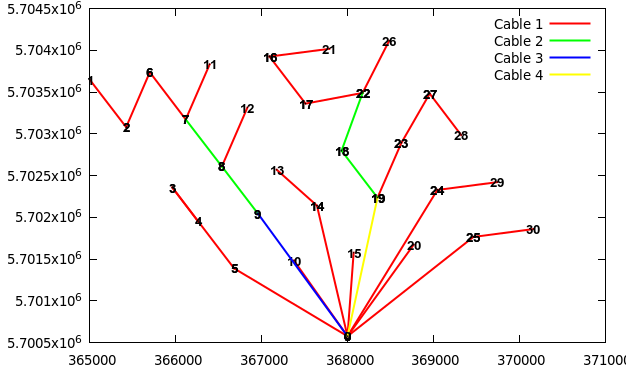
\includegraphics[scale=0.3]{Graphics/1opt-1.png} \\
	\captionof{figure}{Example 1-opt operation step 1}
	\label{img:1opt1}
	\end{minipage}
	\begin{minipage}{7cm} 
	\centering
	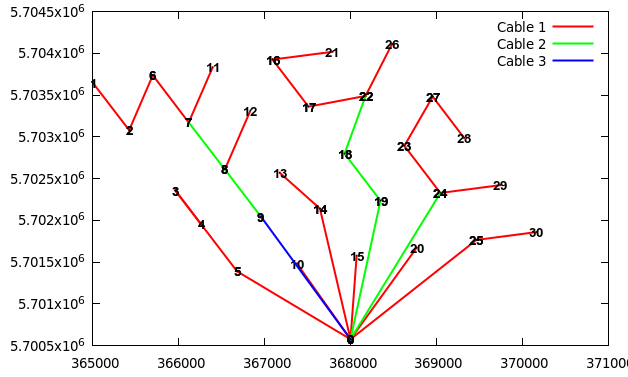
\includegraphics[scale=0.3]{Graphics/1opt-2.png} \\
	\captionof{figure}{Example 1-opt operation step 2}
	\label{img:1opt2}
	\end{minipage}

\newpage
\section{Tabu Search}
Tabu search, proposed by Fred Glover in 1986 and formalized in 1989 [\cite{glover1989tabu}], is a metaheuristic search method that guides a local search procedure to explore the solution space beyond local optimality. \\
In our algorithm Tabu search means to make a move and consider the opposite move \textit{"Tabu"}. In this way the algorithm tries to avoid a local optimum.\\
In our implementation the algorithm start from Prim-Dijkstra solution and applies a \textit{1-OPT} local search until a local optimum is reached. Then, to try to "escape" from the local optimum, the algorithm marks the latest moves \textit{Tabu}. At each move, whether it is improving or worsening the previous solution, the algorithm stores the edges that are involved in the exchange in a data structure, marking them as \textit{Tabu}, which means that they can not be involved again in the future moves. The new move cannot be a move present in the Tabu list. This type of memorization, called \textit{recency-based memory}, keeps track of solution attributes that have changed during the recent past.\\
The capacity of the algorithm to go away from the local optimum is determined by the number of moves that the memory structure can store, and it directly influences the diversification stage. This parameter, called \textit{tabu tenure}, is really difficult to decide a-priori for two reasons: if the \textit{tabu tenure} is large then the risk is to "freeze" the algorithm, because only few moves are allowed and, if it is too small then it will is not assure that the algorithm can escape from all the local optima. So, the choice of \textit{tabu tenure} needs to be tuned through some runs of the algorithm, depending on the instance that has to be solved. We defined a variable \textit{tabu tenure} that starts from 10 and each time the algorithm stops in a local optimum is increased by 10 until it reaches 70. At that moment the Tabu table likely contains too many moves, so we reset the tenure to 10. As we can see in the plot below, the solution improves even if sometimes makes bad moves caused by the Tabu list.

\begin{center}
	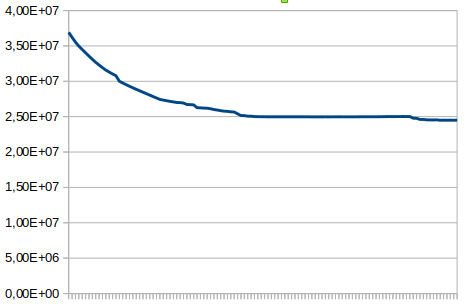
\includegraphics[scale=0.5]{Graphics/graph.png}
	\captionof{figure}{Solution cost history in Tabu search algorithm}
	\label{img:wfcp}
\end{center}

\newpage
\section{Ant Colony Algorithm}
Ant Colony Optimization (ACO) is a heuristic optimization algorithm . The main idea is to follow what the ants do when they find food. An ant moves randomly leaving pheromones: if they do not find anything on the path then the pheromones decay over time. When they finds food, they take it and return to their anthill. They then retrace the path that they previously took, doubling the normal quantity of pheromones. The more pheromones on the path the higher the chance that a new ant follows this path. When another ant follows this path, it reinforces the line of pheromones.\\
With this same logic we can create algorithm (\ref{alg:Ant}) for our problem. Initially every edge of the solution is chosen with the same probability, starting from this solution the algorithm simulates the leaving of pheromones, incrementing the probability of the edges chosen in base on the quality of solution and decreasing the other edges of a fixed percentage to simulate the decay over the time of pheromones. Then the algorithm repeats the choice of the solution basing on the new probability. Doing so, after some repetition of the loop the probability to choose an edge of the optimal solution should be greater than the other edges.\\

\begin{algorithm}
\caption{: Ant Colony Optimization} \label{alg:Ant}
\begin{algorithmic} 
\STATE{\textbf{Input:} Graph $G = (E, V )$, function cost: $P(E) \rightarrow {\rm I\!R}$}
\STATE{\textbf{Data:} Pheromone Values $P_E : E \rightarrow {\rm I\!R}$, Current solution $C \subseteq $}
\STATE{\textbf{Output:} $S \subseteq E$}
\STATE {Initialize pheromone values}
\REPEAT
\STATE {\quad $C \leftarrow$ \textsc{findPath}$(G, P_E)$}
\STATE {\quad $P_E \leftarrow$ \textsc{updatePheromones}$(C, P_E)$}
\STATE {\quad \textbf{if} cost($C$) < cost($S$) \textbf{then}}
\STATE {\quad \quad $S \leftarrow C$}
\UNTIL {\textit{time limit reached}}
\STATE {return $S$}
\end{algorithmic}
\end{algorithm}

There are a lot of ways to implements the logic of the algorithm as we have found in [\cite{nedlin2017ant}], every method for our problem is based on how is implemented the findPath function. We have chosen to implement the ant colony algorithm based on the Kruskal’s algorithm. \\
The Kruscal algorithm [\cite{kruskal1956shortest}] is meant to find the minimum spanning tree, that links all nodes and that has the sum of the weight of its edges as the minimum. The main idea is to order the edges with the increasing weights and choose the new edge to add to the tree that has the minimum cost and does not make cycles with the already selected edges.\\
We implemented the Ant algorithm in the Kruskal approach: as a basis we used again the basic ACO algorithm, but with a modified FindPath function. In this approach we selected the new arc to add to the tree. So first we choose randomly a node, and then we select, using the probability given by the pheromones, an outer arc from the node chosen. The outer arc must satisfy some conditions:
\begin{enumerate}
\setlength{\parskip}{0pt}
\setlength{\itemsep}{0pt plus 1pt}
\item Does not cross, this condition can be forced if there aren’t others choice
\item Does not induces any cycles
\end{enumerate}
This operation repeats until all nodes are linked.

\begin{algorithm}[H]
\caption{: FindPath in Kruskal Approach} \label{alg:SC}
\begin{algorithmic} 
\STATE{\textbf{Input:} Graph $G = (E, V )$, Pheromone Values $P_E$}
\STATE{\textbf{Data:} Current Node $c$, Choice List $L$}
\STATE{\textbf{Output:} $T \subseteq E$}
\REPEAT
\STATE {\textsc{L.CLEAR()}}
\STATE {// select all valid neighbors}
\STATE {\textbf{forall} $(c,v) \in E \smallsetminus \{ e \in E \ | \ T \bigcup \ \{ e \}$ \textit{ contains a circle} \} \textbf{do}} 
\STATE {\quad \textbf{if} \textit{c or v are not connected to a substation in ($V,T$)} \textbf{then}}
\STATE {\quad \quad \textsc{L.INSERT}\textit{(c, v)}}
\STATE {\textbf{if} $L$ \textit{is not empty} \textbf{then}}
\STATE {\quad Select a random edge e = \{ $c,v$ \} from $L$ using $P_E$ as weight}
\STATE {\quad $T \leftarrow T \ \bigcup \ \{ e \}$}
\UNTIL {$L$ \textit{is empty}}
\end{algorithmic}
\end{algorithm}

\section{Results}
In Table 6 we can see the result obtained with the Tabu search, the ant algorithm and the GRASP. The ant algorithm, except in few cases, has the worst results.\\
As we can see, this method does not work very well, this is because with not enough iterations an edges that is in the optimal solution could have a low level of pheromones caused by the fact that the edge could be chosen in bad solutions derived by the choice of other edges, therefore it remains penalized.\\
As to the Tabu search and the GRASP methods, the Tabu search has the best result, also because the GRASP is almost rudimentary (we have implemented it as a Dijkstra algorithm with the variation introduced by GRASP strategy and use 1-Opt move to decrease the objective function). If we compare the Tabu search with the Hard Fixing with the RINS strategy we can see that the Hard Fixing has the best results, but the results are not so different hence the Tabu search is still a good method.\\

\begin{table}[]
\caption{Heuristic methods results ran for 10 minutes}
\begin{tabular}{llll}
\hline
Instance & \textbf{Taboo Search} & \textbf{GRASP $\qquad$} & \textbf{Ant Algorithm} \\ \hline
         & solution              & solution       & solution               \\ \hline
data\_01 & 2.22E+07              & 1.40E+12       & 2.24E+08               \\
data\_02 & 2.42E+07              & 1.30E+12       & 2.62E+07               \\
data\_03 & 2.65E+07              & 1.02E+14       & 2.85E+07               \\
data\_04 & 2.96E+07              & 1.35E+14       & 3.20E+07               \\
data\_05 & 2.73E+07              & 9.02E+11       & 2.30E+08               \\
data\_06 & 2.71E+07              & 1.20E+12       & 2.97E+07               \\
data\_07 & 9.53E+06              & 4.18E+08       & 9.78E+06               \\
data\_08 & 9.31E+06              & 1.01E+11       & 9.50E+06               \\
data\_09 & 1.10E+07              & 6.04E+11       & 2.13E+08               \\
data\_10 & 1.19E+07              & 3.01E+11       & 1.22E+07               \\
data\_12 & 8.93E+06              & 1.01E+11       & 1.00E+07               \\
data\_13 & 9.65E+06              & 1.02E+09       & 9.51E+06               \\
data\_14 & 1.07E+07              & 1.94E+07       & 1.08E+07               \\
data\_15 & 1.08E+07              & 3.00E+11       & 1.22E+07               \\
data\_16 & 8.55E+06              & 3.02E+11       & 9.07E+06               \\
data\_17 & 9.15E+06              & 1.01E+11       & 9.59E+06               \\
data\_18 & 9.27E+06              & 1.02E+09       & 9.68E+06               \\
data\_19 & 9.99E+06              & 2.01E+11       & 1.11E+07               \\
data\_20 & 2.03E+11              & 3.79E+13       & 2.02E+11               \\
data\_21 & 2.03E+11              & 6.30E+13       & 2.01E+11               \\
data\_26 & 2.43E+07              & 1.40E+12       & 2.48E+07               \\
data\_27 & 2.55E+07              & 1.30E+12       & 2.57E+07               \\
data\_28 & 2.01E+11              & 1.77E+14       & 2.01E+11               \\
data\_29 & 2.01E+11              & 2.20E+14       & 2.01E+11               \\ \hline
\end{tabular}
\end{table}